\PassOptionsToPackage{bookmarks={true}}{hyperref}
\pdfminorversion=4
\documentclass[mathserif,xcolor={dvipsnames,table}]{beamer}
\mode<presentation>{\usetheme{Warsaw}\usecolortheme{crane}}
\usepackage{centernot}
\usepackage{upgreek}
\usepackage{graphicx}
\usepackage{framed,color}
\usepackage{geometry}
\usepackage{transparent}
\usepackage{tikz}
\usetikzlibrary{shadows}
\usepackage[utf8]{inputenc}
\usepackage[english]{babel}
\usepackage[T1]{fontenc}
\usepackage{lmodern}
\usepackage[babel=true]{microtype}
\usepackage{amsmath}
\beamertemplatenavigationsymbolsempty

\renewcommand{\sfdefault}{cmr}

\definecolor{shadecolor}{rgb}{1,0.8,0.3}

\title{\textbf{Big-$\boldsymbol{\mathcal{O}}$ Ain't What it Used to Be}}
\date{}
\author{CS4803UWS at the\\
Georgia Institute of Technology
}

\begin{document}

{
\setbeamertemplate{background canvas}{%

\includegraphics[width=\paperwidth,height=\paperheight]{images/gt2.jpeg}
}%
\begin{frame}[plain]
\textcolor{white}{
\transparent{0.5}%
\colorbox{black}{\textbf{Big-$\boldsymbol{\mathcal{O}}$ Ain't What it Used to Be}}
}
\vspace{2.7in}
\\
\hfill
\includegraphics[scale=.25]{images/cc-logo.pdf}

\includegraphics[scale=.25]{images/cc-new.pdf}

\includegraphics[scale=.25]{images/cc-share.pdf}
\textcolor{white}{
\\
\hfill \tiny{CC3.0 share-alike attribution}\\
}
\textcolor{white}{
\hfill \scriptsize{copyright \copyright\ 2013}\\
}
\end{frame}
}

\begin{frame}{Asymptotic notation review I}
Asymptotic analysis gives us a means of speaking of arbitrarily large growth,
independently of arbitrarily (but finitely) large costs not associated with
problem size.
\scriptsize{
\begin{center}
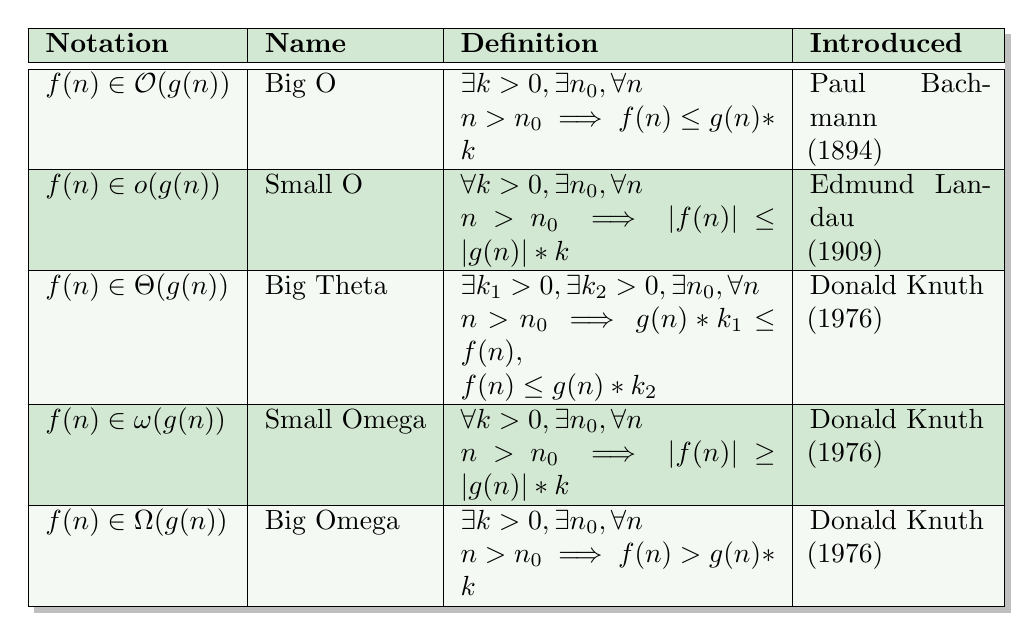
\begin{tikzpicture}
\node[drop shadow,fill=white,inner sep=0pt]
{\rowcolors{1}{ForestGreen!20}{ForestGreen!5}
\begin{tabular}{|l|l|p{4cm}|p{2.25cm}|}
\hline
\textbf{Notation} & \textbf{Name} & \textbf{Definition} & \textbf{Introduced} \\
\hline\hline
$f(n) \in \mathcal{O}(g(n))$ & Big O & $\exists k>0,\exists n_0,\forall n$
\newline
$n>n_0 \implies f(n) \le g(n)*k$ & Paul Bachmann\newline (1894) \\
\hline
$f(n) \in o(g(n))$ & Small O & $\forall k>0,\exists n_0,\forall n$
\newline
$n>n_0 \implies |f(n)| \le |g(n)|*k$ & Edmund Landau\newline (1909) \\
\hline
$f(n) \in \Theta(g(n))$ & Big Theta & $\exists k_1>0,\exists k_2>0,\exists n_0,\forall n$
\newline
$n>n_0 \implies g(n)*k_1 \le f(n),
\newline
f(n) \le g(n)*k_2$ & Donald Knuth\newline (1976) \\
\hline
$f(n) \in \omega(g(n))$ &Small Omega& $\forall k>0,\exists n_0,\forall n$
\newline
$n>n_0 \implies |f(n)| \ge |g(n)|*k$ & Donald Knuth\newline(1976) \\
\hline
$f(n) \in \Omega(g(n))$ & Big Omega & $\exists k>0,\exists n_0,\forall n$
\newline
$n>n_0 \implies f(n) > g(n)*k$ & Donald Knuth\newline (1976) \\
\hline
\end{tabular}%
};
\end{tikzpicture}
\end{center}
\vfill
Advances in (finite) computing technology can only reduce these
ignored costs. Wrap the earth with your register file, and still there will be
numbers so large that their addition is $\Theta(n)$.
}
\end{frame}

\begin{frame}{Asymptotic notation review II}
\scriptsize{
\begin{center}
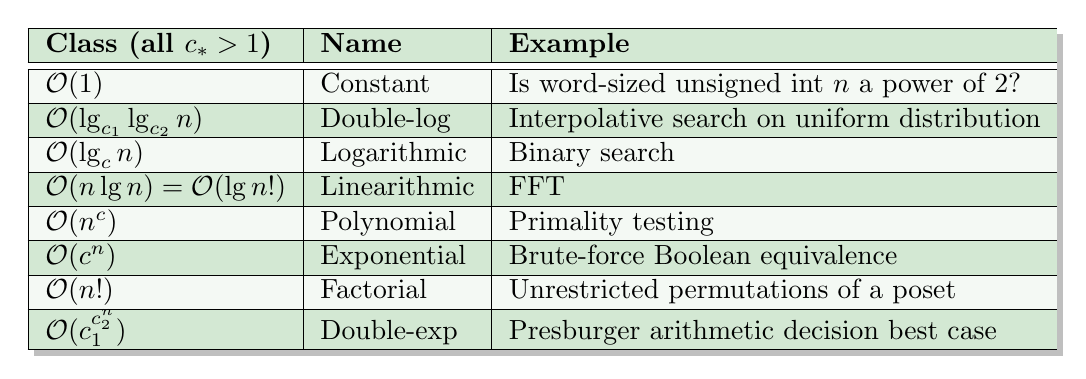
\begin{tikzpicture}
\node[drop shadow,fill=white,inner sep=0pt]
{\rowcolors{1}{ForestGreen!20}{ForestGreen!5}
\begin{tabular}{|l|l|l}
\hline
\textbf{Class (all $c_*>1$)} & \textbf{Name} & \textbf{Example} \\
\hline\hline
$\mathcal{O}(1)$ & Constant & Is word-sized unsigned int $n$ a power of 2?\\
\hline
$\mathcal{O}(\lg_{c_1}\lg_{c_2} n)$ & Double-log & Interpolative search on uniform distribution\\
\hline
$\mathcal{O}(\lg_c n)$ & Logarithmic & Binary search\\
\hline
$\mathcal{O}(n\lg n) = \mathcal{O}(\lg n!)$ & Linearithmic & FFT\\
\hline
$\mathcal{O}(n^{c})$ & Polynomial & Primality testing\\
\hline
$\mathcal{O}(c^{n})$ & Exponential & Brute-force Boolean equivalence \\
\hline
$\mathcal{O}(n!)$ & Factorial & Unrestricted permutations of a poset\\
\hline
$\mathcal{O}(c^{c^{n}_2}_1)$ & Double-exp & Presburger arithmetic decision best case\\
\hline
\end{tabular}%
};
\end{tikzpicture}
\end{center}
\vfill
Speaking of still faster growth rates\footnote{\scriptsize{Check out ``fast-growing hierarchies'' and the L\"ob–Wainer hierarchy.}} (hyper-exponential, $\mathcal{A}(n)$)
 is mostly zoology.%\footnote{\scriptsize{Forgive the pun on busy beavers.}}.
}
\end{frame}

\begin{frame}{It's the constants, stupid}
Algorithmic choices can dominate performance, especially at scale. By the
definition of Big O, it should also be obvious that an asymptotically superior
algorithm can be slower for small inputs\footnote{We will see that small inputs can be surprisingly large.}.\\
\vfill
That said, no one's going to think implementing a routing table with a linked list is a good idea.\\
\vfill
Furthermore, asymptotic analysis speaks of performance as problem size grows.
It doesn't speak of real-time. It doesn't speak of bounded memories.
We rarely speak of piecewise asymptotics.
\vfill
But, by all means, do ensure you're not doing linear searches on sorted data etc.
\end{frame}

\begin{frame}{What's hiding behind $\mathcal{O}$?}
Naive square (nXn X nXn) matrix multiplication is $\Theta(n^{3})$.
\vfill
\begin{equation}
C = AB \implies C_{ij} = \sum\limits_{m=1}^{k} A_{im}B_{mj}
\end{equation}
\vfill
Counting the explicit additions and multiplications, there are
precisely $2n^{3}$ ``operations''.
\end{frame}

\begin{frame}{Fused multiply-add}
\small{
IEEE 754-2008 floating point support requires FMA, fused multiply-add.
Let $rn()$ denote a rounding operation. Typically, a multiply-add chain
requires two instructions, and rounds twice:
\begin{equation}
MAC(A,B,C) = rn(rn(A * B) + C)
\end{equation}
Fused multiply-add rounds only once, preserving the fully precise product in
an internal register:
\begin{equation}
FMA(A,B,C) = rn(A * B + C)
\end{equation}
AMD's FMA4 (Bulldozer) implements a fully general SIMD FP FMA. Intel's FMA3
(Haswell, as part of AVX2; also in AMD's Piledriver) implements a destructive
SIMD FP FMA\footnote{AMD's XOP further implements an SIMD integer FMA.}.
The throughput and latency are equivalent to standard single SIMD FP adds and
multiplies. NVIDIA's Fermi likewise introduced a full-throughput FMA.
\vfill
There are now precisely $n^{3}$ ``operations''.
}
\end{frame}


{
\setbeamertemplate{background canvas}{%
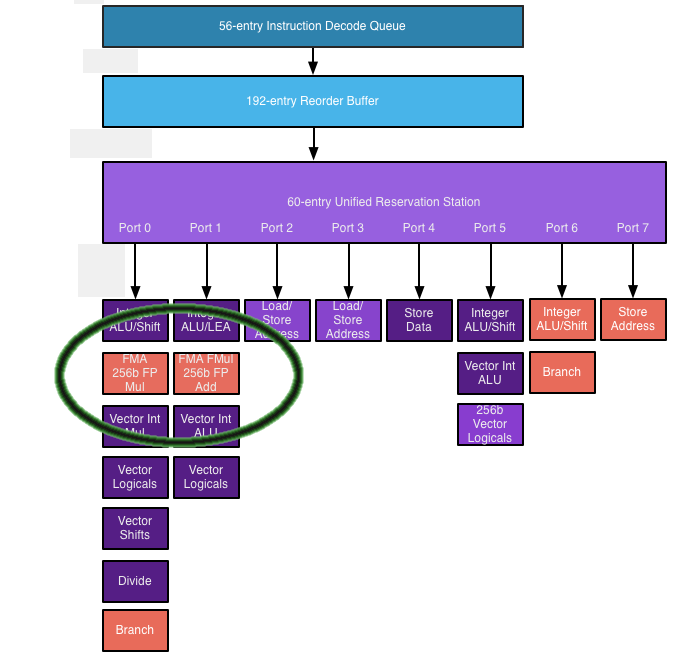
\includegraphics[scale=.33]{images/haswellexec.png}
}%
\begin{frame}[b]{Wide issue}
\scriptsize{
Haswell can issue and retire 2 VFMADD* instructions per cycle.\\
There are now precisely $n^{3}/2$ ``operations''\footnote{\tiny{Assuming that two operations are available every cycle.}}.
\vspace{.1in}
}
\end{frame}
}

{
\setbeamertemplate{background canvas}{%
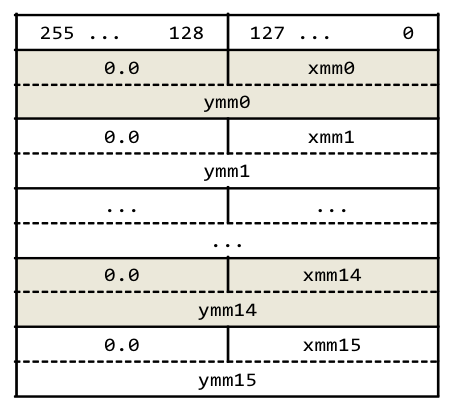
\includegraphics[scale=1]{images/256bit.png}
}%
\begin{frame}[b]{SIMD}
\scriptsize{
AVX uses the 16 256-bit YMM registers. There are 8 32-bit IEEE 754-2008
single-precision values in a 256-bit input.\\
There are now precisely $n^{3}/16$ ``operations''\footnote{Assuming that values
are usable in 256-bit chunks.}.
\vspace{.1in}
}
\end{frame}
}

{
\setbeamertemplate{background canvas}{%
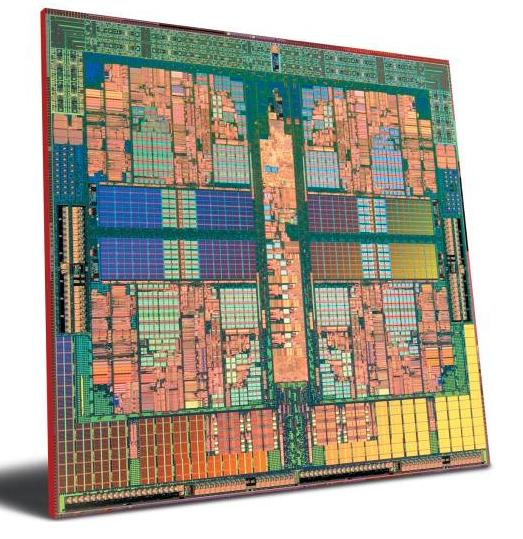
\includegraphics[scale=1]{images/Multicore.jpg}
}%
\begin{frame}[b]{Multicore}
\scriptsize{
\begin{block}{}
Haswell will likely debut in a quadcore physical package.\\
There are now precisely $n^{3}/64$ ``operations''\footnote{\tiny{Ignoring communication
costs, and assuming perfect parallelism.}}.
\end{block}
\vspace{.1in}
}
\end{frame}
}

\begin{frame}{Memory accesses}
\begin{enumerate}
\item $\forall i, 0\le i \le n:$ Read row $i$ from $A$ into $a$
\item $\forall j, 0\le j \le n:$ Read column $j$ from $B$ into $b$, read $C_{ij}$ into $c$
\item $\forall k, 0\le k \le n:$ Store $a_k * b_k + c$ into $C_{ij}$
\end{enumerate}
\vfill
\begin{enumerate}
\item $n^{2}$ loads from A
\item $n^{3}$ loads from B
\item $n^{2}$ loads from C
\item $n^{2}$ stores to C
\end{enumerate}
Counting the loads and stores, there are precisely $n^{3} + 3n^{2}$ memory
accesses. There are now precisely $\frac{65n^{3}}{64} + 3n^{2}$ ``operations''.
\vfill
\begin{alertblock}{Arithmetic intensity}
\center$\lim\limits_{n \to \infty} \frac{\text{Arithmetic}}{\text{Memory}} = 2$
\end{alertblock}
\vfill
\end{frame}

\begin{frame}{Loads and stores}
Hong and Kung proved in 1981 that any schedule of conventional matrix
multiplication must transfer $\Omega(\frac{n^{3}}{\sqrt{Z}}), Z<\frac{n^{2}}{6}$
words between slow and fast memory. \textit{Tiling} is the optimal strategy.
\vfill
Of course, AVX's VMOVAPS moves 256 bits, or 8 32-bit single precision floating
point words, at a time. And there's 4 cores. With two load/store pipes each. So that's $\Omega_{HK}/64$\footnote{
\tiny{Assuming that the values are located in aligned, contiguous 256-bite chunks in memory.\\
\hspace{.6cm}Wait\ldots we can use VMOVUPS if they're unsuitably aligned.}}.
\vfill
Of course, we're not going to be able to pack two VFMADDPS and two VMOVAPS
instructions into every 16B/\textbf{c} I\$ fetch\footnote{\tiny{VEX-encoded
VMOVAPS tends to run \textasciitilde 5 bytes.}}.
\vfill
How does this interact with register banking? Multilevel caching? TLBs? Page
cache? Prefetching? DRAM banking? Multilevel disk? Logical cores? Other physical cores?
NUMA?
\end{frame}

{
\setbeamertemplate{background canvas}{%

\includegraphics[scale=1]{images/rage.jpg}
}%
\begin{frame}{Argh}
\begin{block}{FFFFFFFFFFFFFFFFFFFFFFUUUUUUUUUUUUUUUUUUU}
We've not yet mentioned branching.
\end{block}
\end{frame}
}

\begin{frame}{CS4803 Spring 2010 Lab 3---All $\mathcal{O}(n^{3})$}
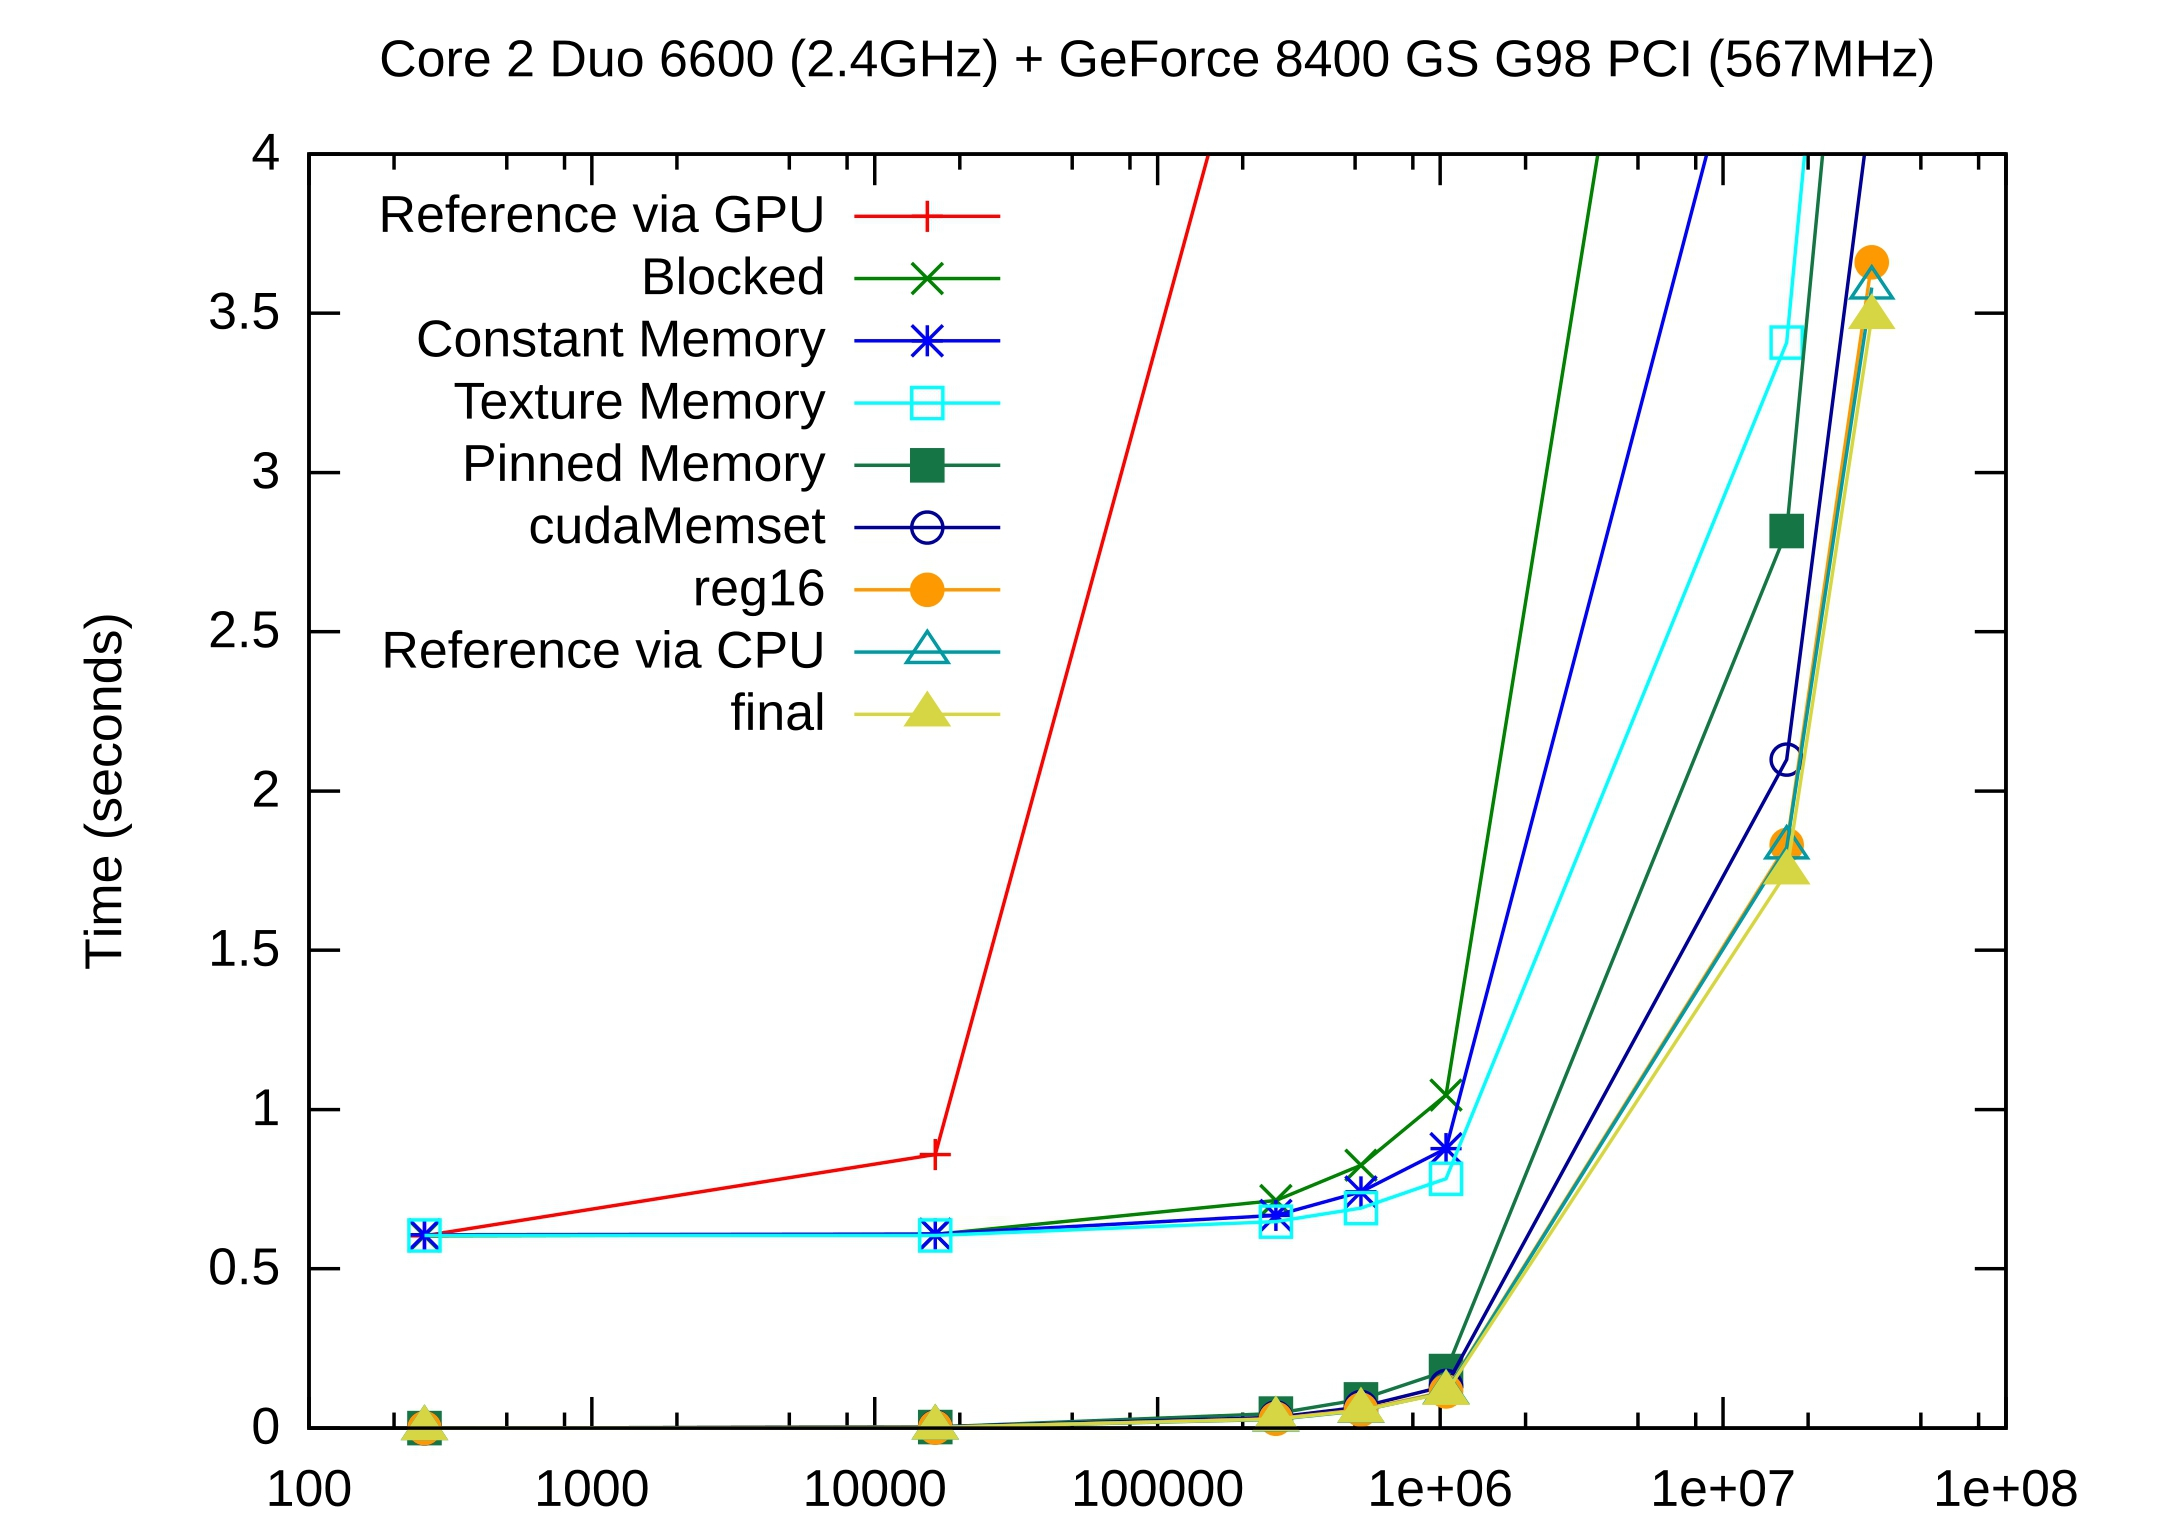
\includegraphics[width=.8\paperwidth]{images/lab3.jpg}
\end{frame}

\begin{frame}{ATLAS Unleashed---All $\mathcal{O}(n^{3})$\hfill\tiny{Image source: Richard Vuduc's CSE6230}}
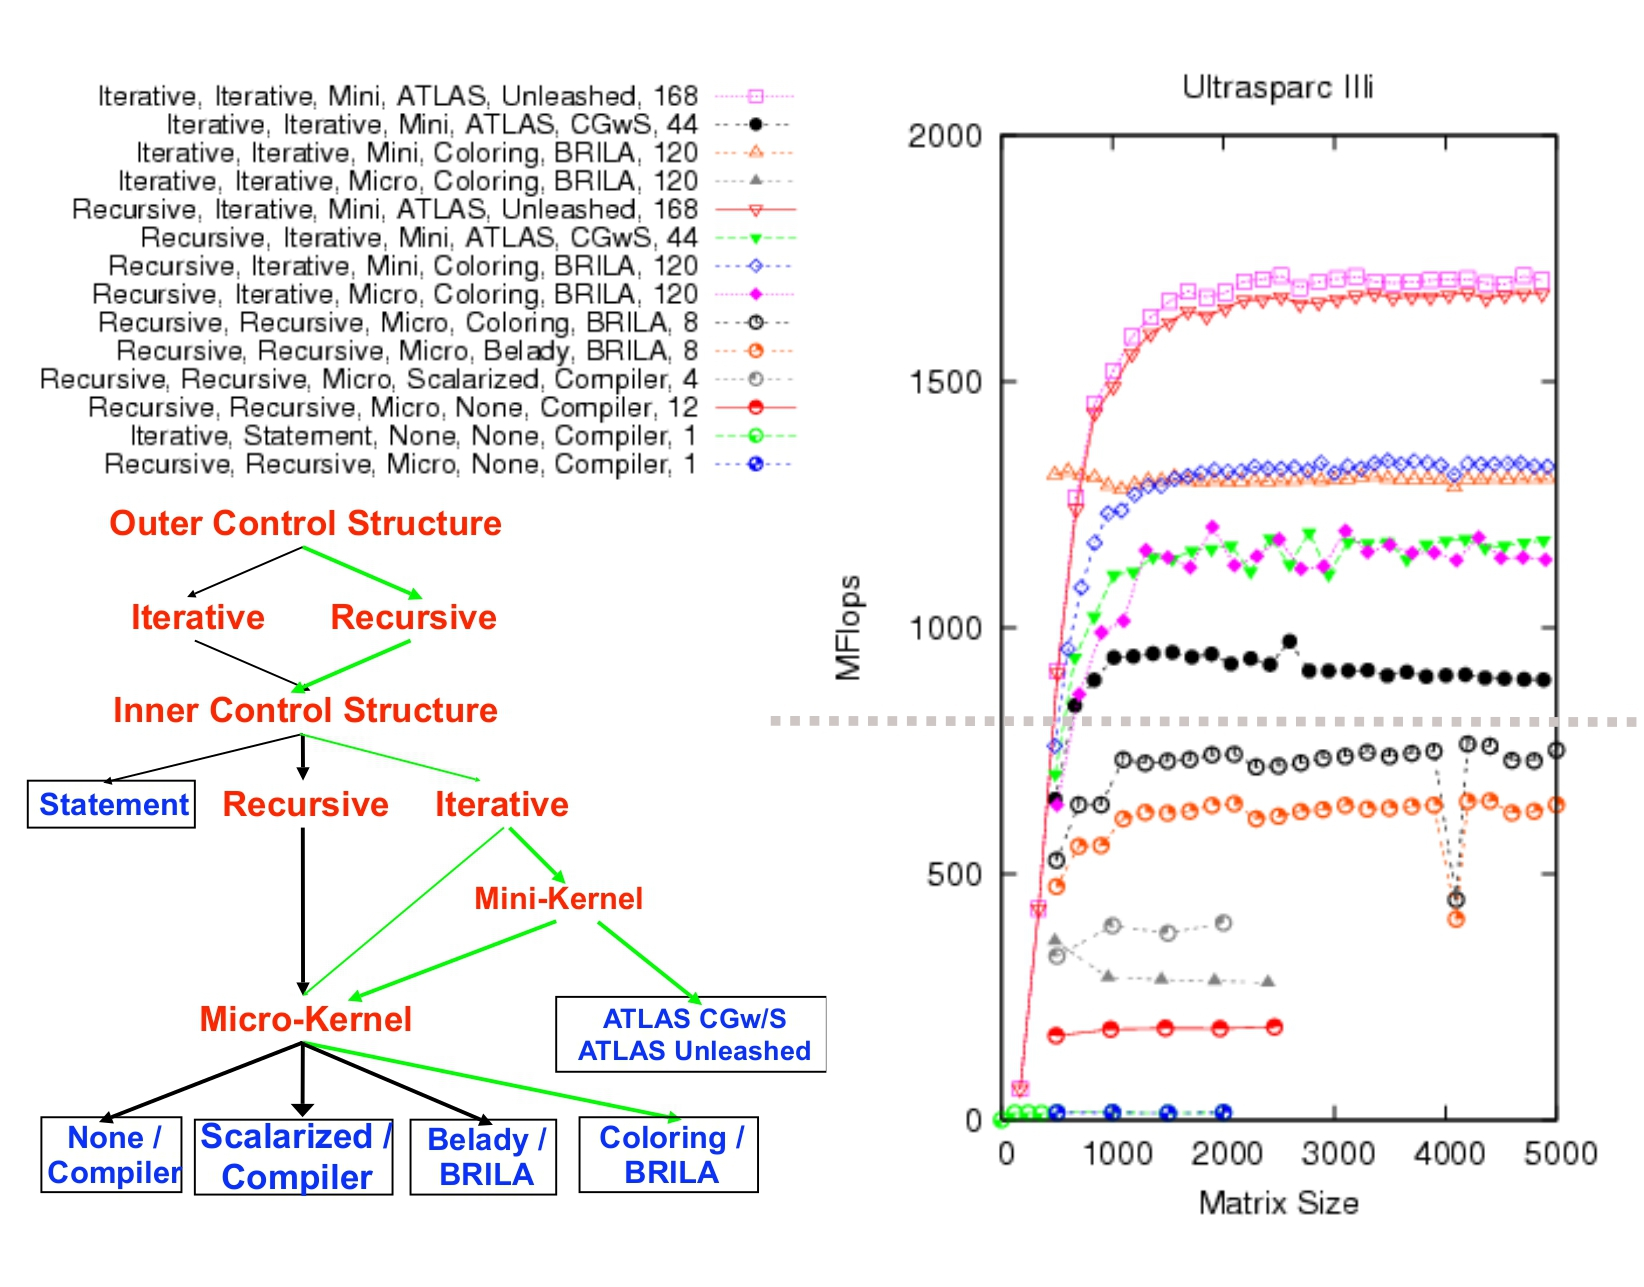
\includegraphics[width=.8\paperwidth]{images/vuduc.jpg}
\end{frame}

\begin{frame}{RAPTORIAL-file\hfill\tiny{Image source: Dirty South Supercomputing and Waffles}}
\begin{center}
In the pure systems space, $\mathcal{O}$ makes still less sense.\\
What's $\mathcal{O}$ of multithreaded file lexing?\\
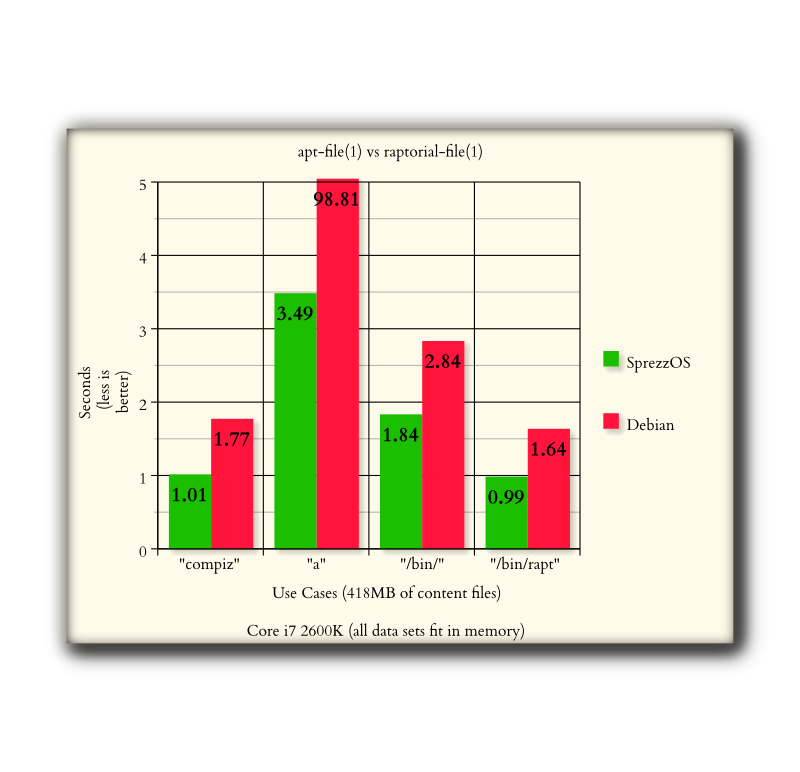
\includegraphics[width=.675\paperwidth]{images/raptorial-file-fullsize.png}
\end{center}
\end{frame}

\begin{frame}{RAPT-show-version\hfill\tiny{Image source: Dirty South Supercomputing and Waffles}}
\begin{center}
Nonetheless, optimization can be very fruitful.
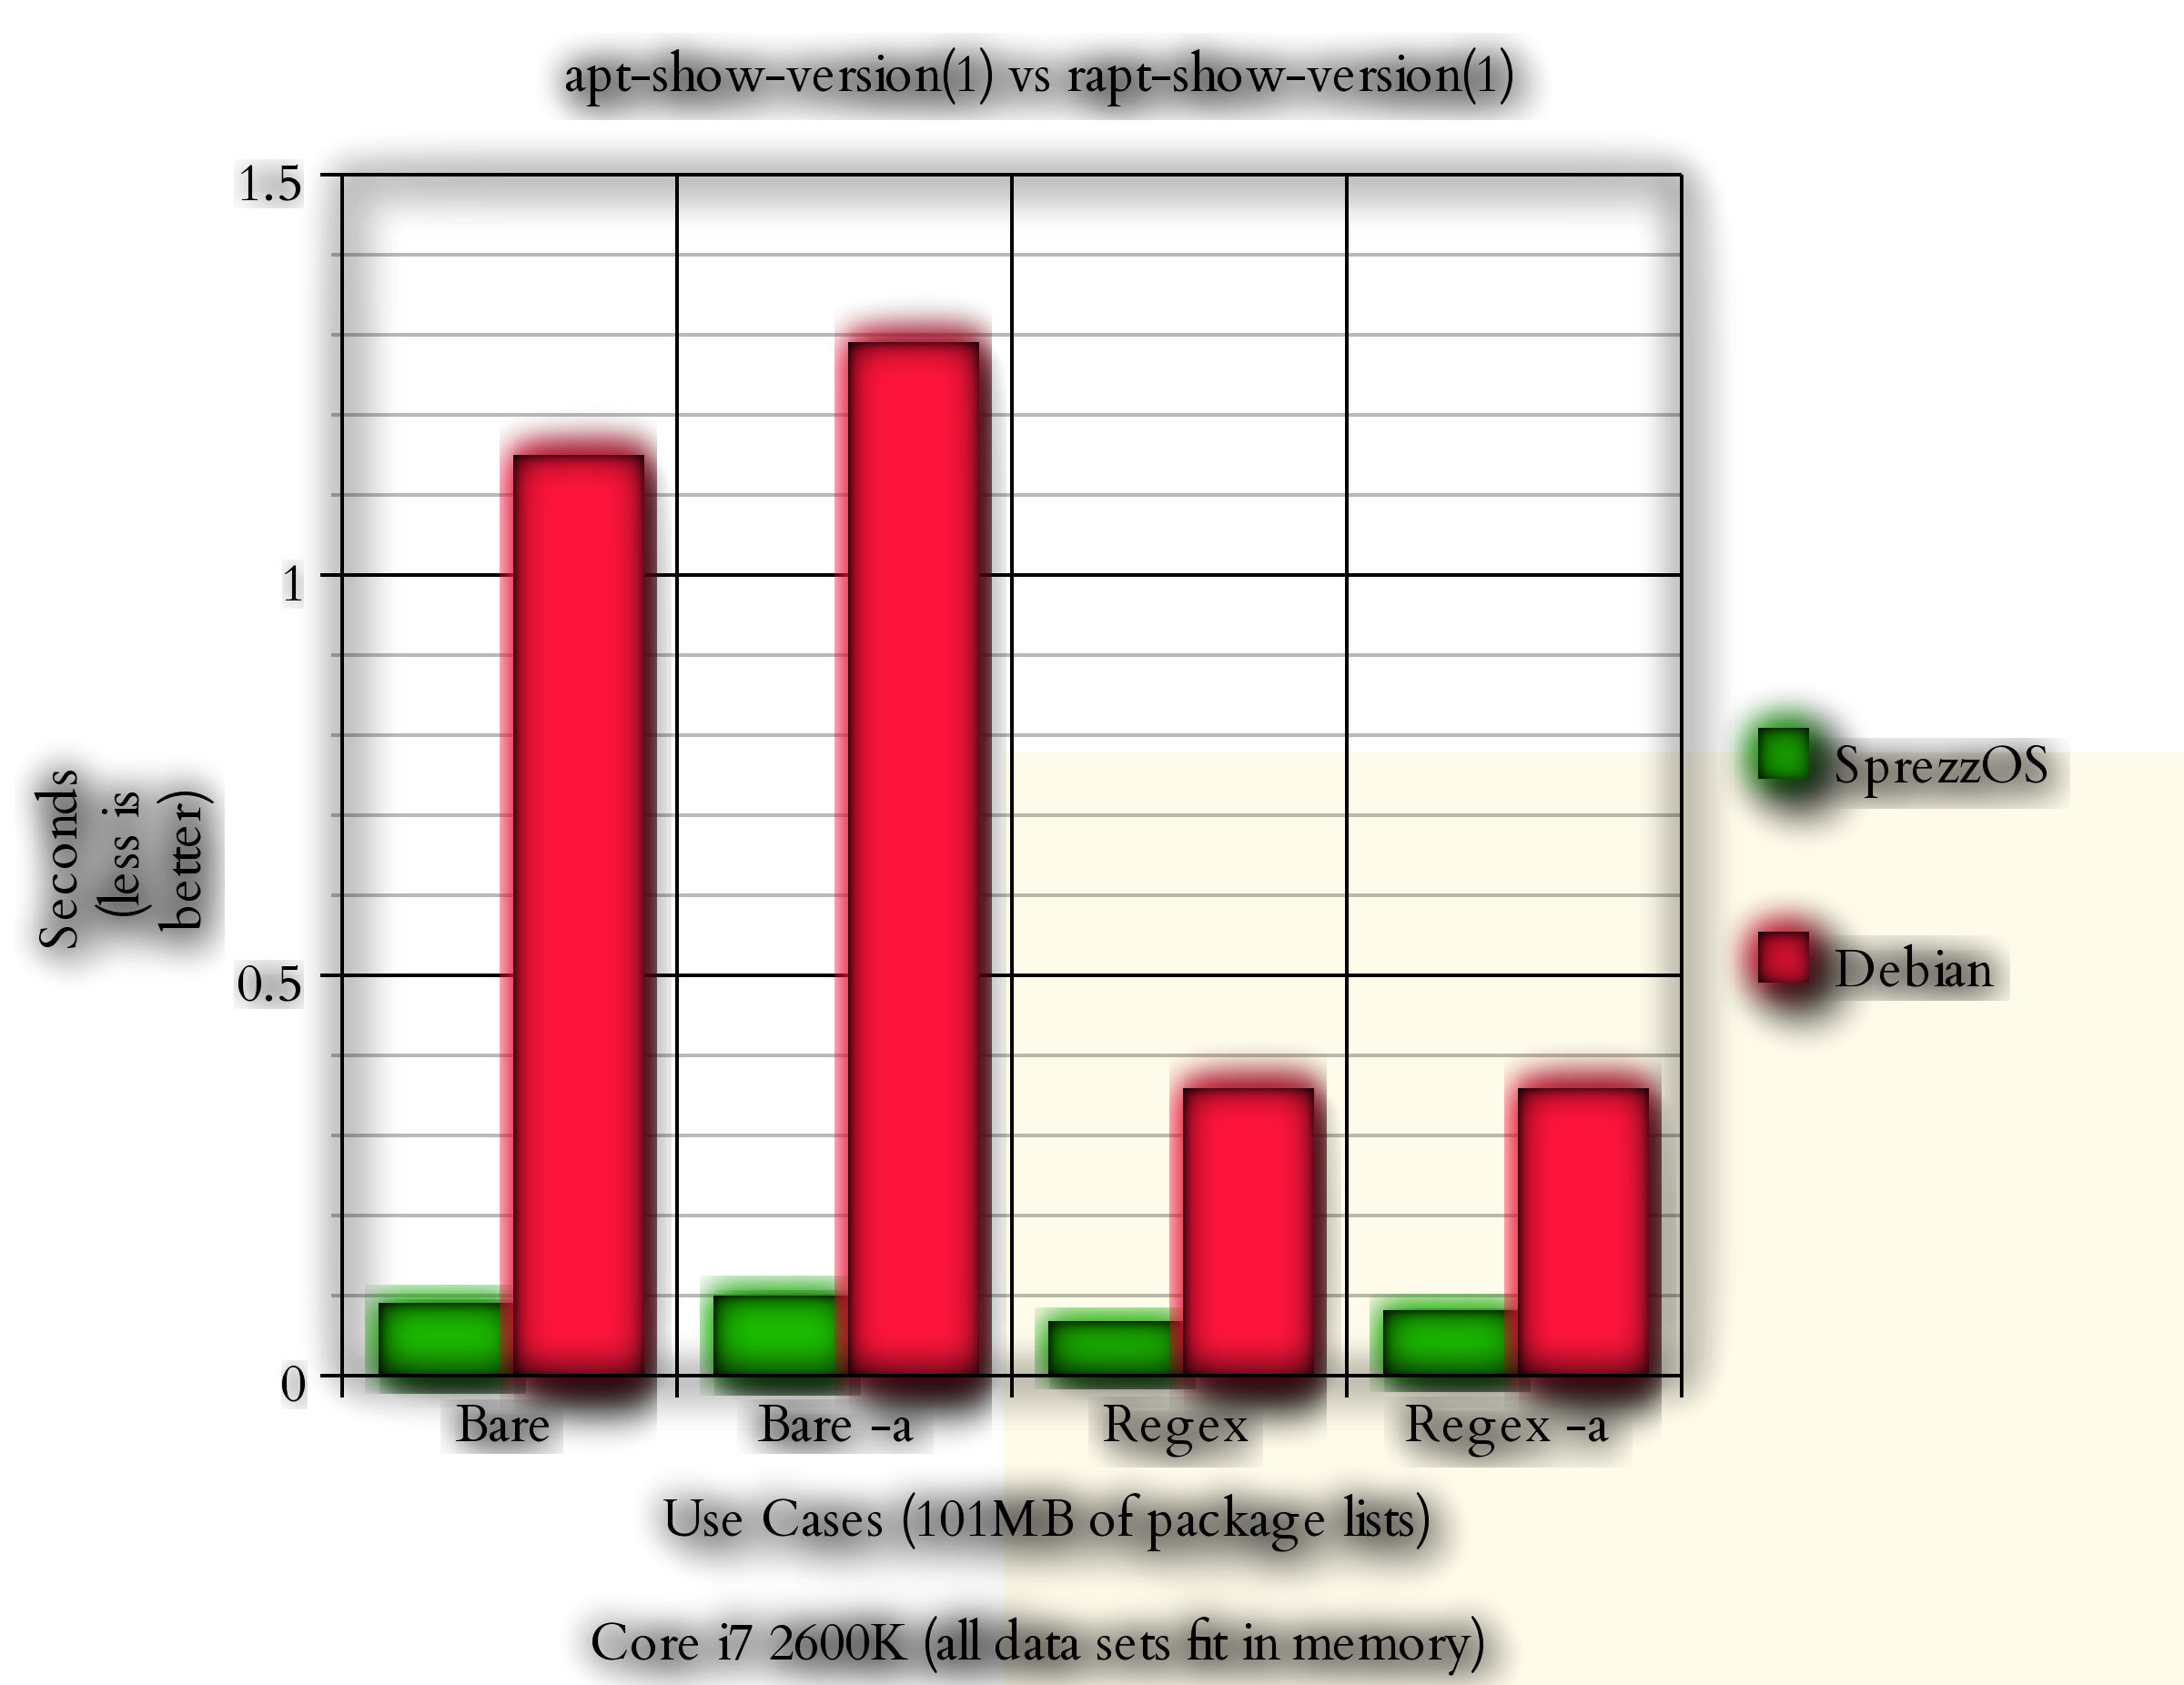
\includegraphics[width=.675\paperwidth]{images/rapt-show-versions-fullsize.png}
\end{center}
\end{frame}

{
\setbeamertemplate{background canvas}{%
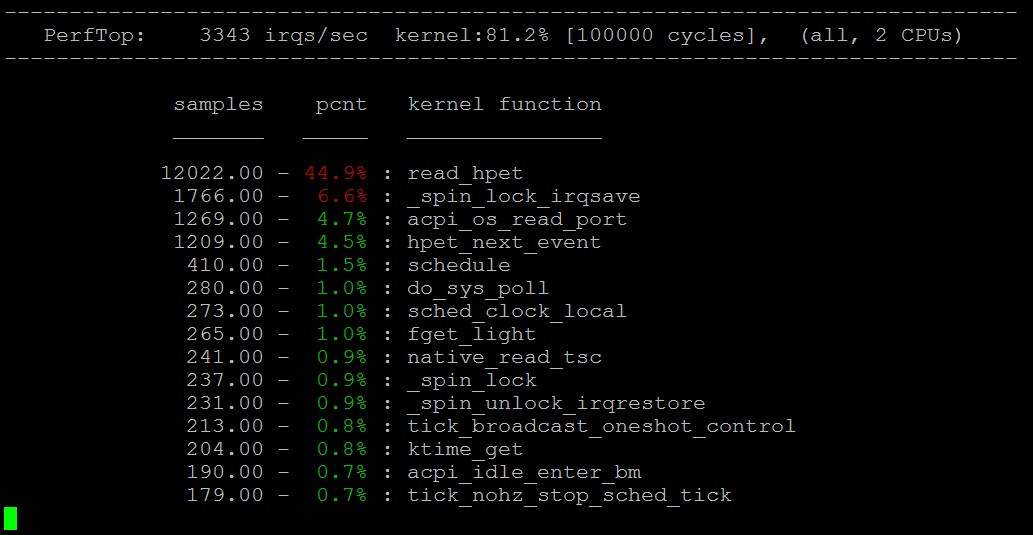
\includegraphics[scale=.5]{images/perf1.jpg}
}%
\begin{frame}[b]{Analysis-driven optimization I}
\begin{block}{High-level (``Macroanalysis'')}
Coarse tools and algorithmic reasoning, e.g.:
\begin{itemize}
\item Ensure sufficient task-level parallelism
\item Ensure cores aren't overutilized
\item Profiler-driven hotspot location
\item High-level memory and I/O flow
\end{itemize}
\end{block}
\end{frame}
}

{
\setbeamertemplate{background canvas}{%
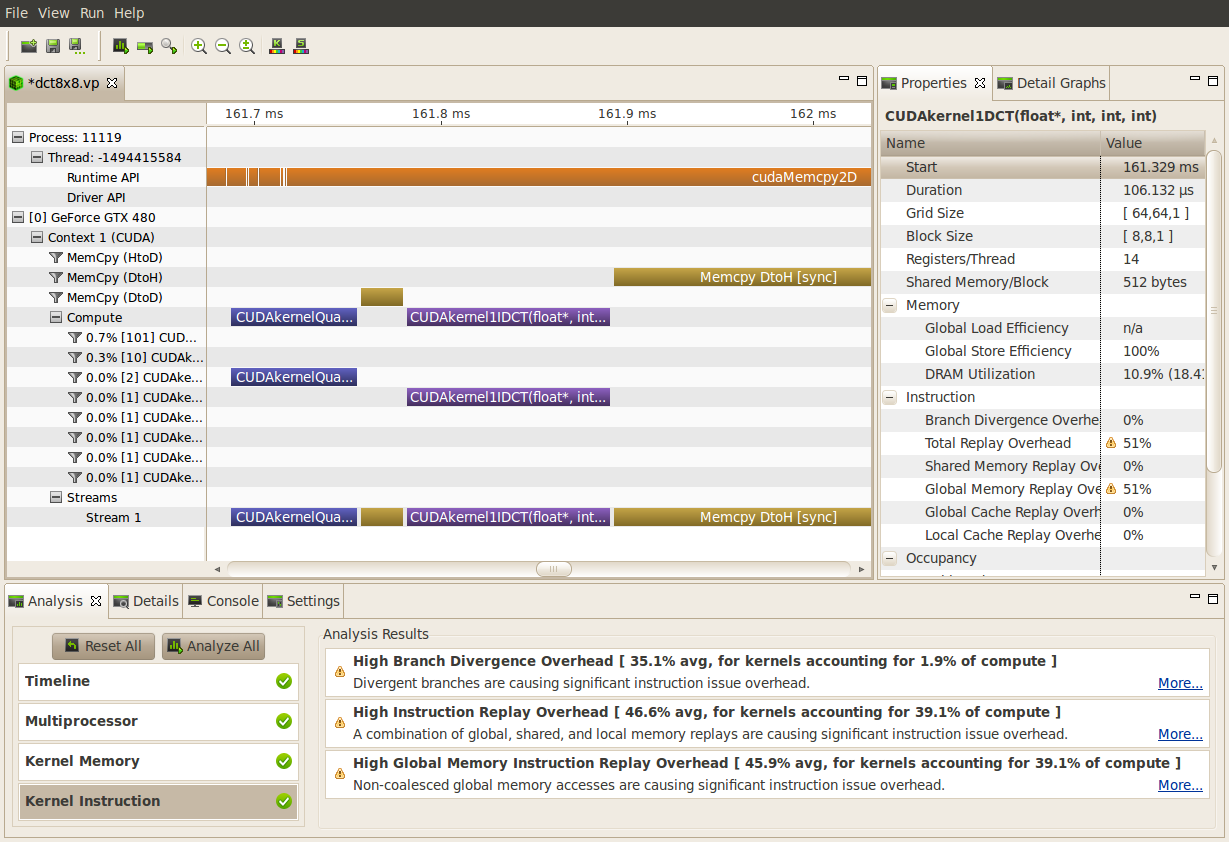
\includegraphics[width=\paperwidth]{images/cudaprof.png}
}%
\begin{frame}[b]{Analysis-driven optimization II}
\begin{block}{Low-level (``Microanalysis'')}
Performance counters and throughput-based reasoning, e.g.:
\begin{itemize}
\item Vectorize
\item Tune for caches
\item Watch for $\upmu$architectural stalls
\end{itemize}
\end{block}
\end{frame}
}

\begin{frame}{Complexity finds a way}
\begin{center}
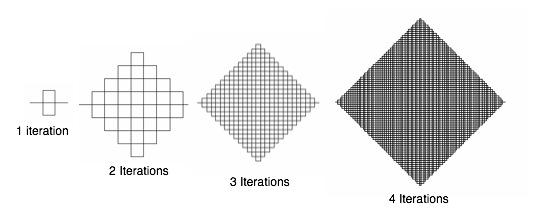
\includegraphics[width=\textwidth]{peano.jpg}\\
\tiny{A fractal having Hausdorff dimension 2,\\
the space-filling Peano curve is used in cache-oblivious algorithms.}
\end{center}
\vfill
\large{\textbf{Mastering the complex modern design space requires deftly
switching between theoretical analysis, guided experiment, and pure
exploration.\\
\vspace{.25in}
This class is about doing so.}}
\end{frame}

%In terms of pure growth, we have $ijk$, so we can set
%\begin{equation}
%n=\frac{i}{3} + \frac{j}{3} + \frac{k}{3}
%\end{equation}
%and this is a very accurate analysis.
%Do you see $n$?\\
%\vfill
%I see $k$ additions of $k$ multiplications, done $i * j$ times. So $n$ is the
%average of our three sizes. But really, $k$ contributes twice as much as either
%$i$ or $j$. So
%\begin{equation}
%n = \frac{k}{2} + \frac{i}{4} + \frac{j}{4}
%\end{equation}
%
%naively, a bit at a time on $b$-bit inputs, I see $ijk\Theta(b) + ijk\mathcal{O}(b^{2})
%\implies ijk\mathcal{O}(b^{2})$. Fix $b$. I see $ijkb + ijkb^{2}$. What, we can add
%$b$-bit words in a single operation? I see $ijk + ijkb$
%\footnote{\tiny{Note that whatever $b$ we pick, so long as we pick a finite $b$, the
%asymptotic analysis holds---whether $b$ or $b^{2}$, it's just a constant factor
%as our problem grows. Accurately multiplying matrices of fixed size, but having arbitrarily
%large elements, is a different analysis.}}
%. Ho ho, we have a hardware
%multiplier? $ijk + ijk$ it is!

\begin{frame}{Recommended reading}
\tiny{
\begin{itemize}
\item Hong and Kung. ``I/O complexity: The red-blue pebble game'' (1981).
\item Yotov et al. ``An experimental comparison of cache-oblivious and cache-conscious programs'' (2007).
\item Irony et al. ``Communication Lower Bounds for Distributed-Memory Matrix Mul'' (2004).
\item Goto et al. ``Anatomy of High-Performance Matrix Multiplication'' (2008).
\item Kalyanasundaram et al. ``Improved Simulation of NTMs'' (2011).
\item Fran\c{c}ois Le Gall. ``Faster Algorithms for Rectangular Matrix Multiplication'' (2012).
\item Eric Quinnell. ``Floating-Point Fused Multiply-Add Architectures'' (2007).
\item Tom Leighton. ``Better Master Theorems for Divide-and-Conquer Recurrences'' (1996).
\item \textit{Intel Instruction Set Extensions Programming Reference}
\end{itemize}
}
\end{frame}

%\begin{frame}{Hack on!}
%\end{frame}

\end{document}
